\documentclass[ignoreonframetext,unicode,aspectratio=169]{beamer}
%

\usepackage[utf8]{inputenc}
\usepackage[T1]{fontenc}
\usepackage[english,russian]{babel}
\usepackage{amsmath}
\usepackage{amsfonts}
\usepackage{amssymb}
\usepackage{graphicx,pgf}
\usepackage{multimedia}
\usepackage{relsize}
\usepackage{mathtools}
\usepackage{multirow}
\usepackage{hyperref}
\usepackage{listings}
\usepackage{appendixnumberbeamer}

\usetheme{Warsaw}

\setbeamertemplate{caption}[numbered]

\useinnertheme{circles}
\usecolortheme{rose}

\newcommand{\size}{0.36}
\setbeamertemplate{caption}{\insertcaption}

% номера слайдов
\newcommand*\oldmacro{}%
\let\oldmacro\insertshorttitle%
\renewcommand*\insertshorttitle{%
	\oldmacro\hfill%
	\insertframenumber\,/\,\inserttotalframenumber}
\RequirePackage{caption}
\DeclareCaptionLabelSeparator{defffis}{ }
\captionsetup{justification=centering,labelsep=defffis}

% Картинки ищем в подпапке animation/ (как в исходной презентации)
\graphicspath{{animation/}{./}}

% Название приведено к теме ВКР
\title[Моделирование УВ с локальным энерговложением (JAX)]{Моделирование распространения ударной волны в газе с локальным энерговложением средствами библиотеки JAX}
\author[Филькин Д.\,С.]{Докладчик: Филькин Д.\,С.\and\\[0.5mm] Научный руководитель: Кравченко О.\,В.}
\institute[каф. Прикладная математика ФН-1]{группа ФН1-81Б}
\date{\today} % TODO: поставить дату защиты
\titlegraphic{
\includegraphics[width=2 cm]{logo.png}}

\begin{document}

	\begin{frame}[plain]
		\maketitle
	\end{frame}

	%==================================================================
	% Слайд: Актуальность и мотивация
	\begin{frame}{Мотивация и цели исследования}

%		\begin{block}{Физическая проблематика}
%			\begin{itemize}
%				\item \textbf{Взаимодействие УВ с неоднородностями:} исследуется прохождение ударной волны (УВ) через зону \textbf{локального энерговложения} --- область пониженной плотности, моделирующую подвод энергии в газ.
%			\end{itemize}
%		\end{block}

		\begin{alertblock}{Мотивация}
			Для выявления физических закономерностей динамики ударной волны требуется проведение параметрического исследования с    параметром разрежения $\alpha$
		\end{alertblock}
		
		\begin{block}{Цель работы}
			Численное моделирование распространения ударной волны в газе с локальным энерговложением средствами разработанного высокопроизводительного программного комплекса на базе библиотеки JAX.
		\end{block}
		
%		\vspace{0.2cm}
		
		\textbf{Основные задачи:}
		\begin{itemize}
			\item Высокопроизводительная реализация центральных схем высокого разрешения SD2 и FD2 средствами JAX,
			\item кросс-верификация решения относительно библиотек \texttt{centpy} и \texttt{JAX-FLUIDS},
			\item анализ аппаратного ускорения на CPU и GPU,
			\item демонстрация возможностей комплекса на задаче о прохождении УВ через зону энерговложения в 1D и 2D.
		\end{itemize}

	\end{frame}
	
	%==================================================================
	% Слайд: Библиотека JAX
	\begin{frame}{Библиотека JAX --- инструмент реализации}
		\begin{columns}[t]
			\begin{column}{0.46\textwidth}
				\begin{block}{Что такое JAX}
					\texttt{JAX} --- библиотека для высокопроизводительных численных вычислений: NumPy-совместимый API (\texttt{jax.numpy}) с компиляцией под CPU, GPU и TPU \textbf{из единого кода}.
				\end{block}
				\begin{block}{Почему именно она}
					Один и тот же решатель без изменения кода исполняется и на CPU, и на GPU --- это даёт серийные расчёты, необходимые для параметрического исследования по $\alpha$.
				\end{block}
			\end{column}
			\begin{column}{0.54\textwidth}
				\begin{block}{Возможности, использованные в комплексе}
					\begin{itemize}
						\item \textbf{JIT-компиляция} (\texttt{jax.jit}\,$\to$\,XLA): шаг по времени компилируется в слитное ядро --- основной источник ускорения;
						\item \textbf{функциональный стиль}: чистые функции и неизменяемые массивы; обновление через \texttt{x.at[i].set(...)};
						\item \textbf{\texttt{lax.while\_loop}}: компилируемый цикл интегрирования с динамическим числом шагов;
						\item \textbf{двойная точность} (\texttt{x64}) --- для корректной аппроксимации.
					\end{itemize}
				\end{block}
			\end{column}
		\end{columns}
\end{frame}
	
	
		\begin{frame}{Центральные схемы второго порядка}
		\begin{columns}[t]
			%--- SD2 (полудискретная, Кургáнова--Тадмора) ---
			\begin{column}{0.5\textwidth}
				\centering\textbf{SD2 --- полудискретная}\par
				\vspace{0.1 cm}
				\footnotesize
				\begin{block}{Реконструкция:}
					\[
					\begin{aligned}
						u^\mp_{i\pm1/2} = u_i \pm \tfrac12\,\text{minmod}\big(&u_i-u_{i-1},\\[-3pt]
						&u_{i+1}-u_i\big)
					\end{aligned}
					\]
				\end{block}
				\vspace{-0.2 cm}
				\begin{block}{Численный поток:}
					\[
					\begin{aligned}
						H_{i+1/2}=\tfrac12\big(&f(u^+_{i+1/2})+f(u^-_{i+1/2})\\[-3pt]
						&-\,a_{i+1/2}(u^+_{i+1/2}-u^-_{i+1/2})\big)
					\end{aligned}
					\]
				\end{block}
				\vspace{-0.2 cm}
				\begin{block}{Полудискретная ОДУ:}
					\[
					\frac{d u_i}{dt}=-\frac{H_{i+1/2}-H_{i-1/2}}{\Delta x}
					\]
					\centering{\scriptsize интегрирование по времени --- SSP-RK2}
				\end{block}
			\end{column}
			%--- FD2 (полностью дискретная, Несьяху--Тадмора) ---
			\begin{column}{0.5\textwidth}
				\centering\textbf{FD2 --- полностью дискретная}\par
				\vspace{0.1 cm}
				\footnotesize
				\begin{block}{Наклоны (minmod):}
					\[
					\begin{aligned}
						u'_i &= \text{minmod}(u_i-u_{i-1},\,u_{i+1}-u_i)\\[-3pt]
						f'_i &= \text{minmod}(f_i-f_{i-1},\,f_{i+1}-f_i)
					\end{aligned}
					\]
				\end{block}
				\vspace{-0.2 cm}
				\begin{block}{Предиктор:}
					\[
					u_i^{\,n+1/2}=u_i^{\,n}-\frac{\Delta t}{2\Delta x}\,f'_i
					\]
				\end{block}
				\vspace{-0.2 cm}
				\begin{block}{Корректор (шахматная сетка):}
					\[
					\begin{aligned}
						u_{i+1/2}^{\,n+1}=&\tfrac12\big(u_i^{\,n}+u_{i+1}^{\,n}\big)+\tfrac18\big(u'_i-u'_{i+1}\big)\\[-3pt]
						&-\frac{\Delta t}{\Delta x}\big(f(u_{i+1}^{\,n+1/2})-f(u_i^{\,n+1/2})\big)
					\end{aligned}
					\]
				\end{block}
			\end{column}
		\end{columns}
	\end{frame}

	%==================================================================
	% Слайд: Математическая постановка (E -> rho E)
	\begin{frame}{Одномерная постановка задачи}

		\begin{block}{Система уравнений Эйлера}
			\[
			\partial_t \begin{pmatrix} \rho \\ \rho u \\ \rho E \end{pmatrix} +
			\partial_x \begin{pmatrix} \rho u \\ \rho u^2 + p \\ (\rho E + p)u \end{pmatrix} = 0
			\]

			с уравнением состояния идеального газа
			\vspace{-0.3 cm}
			\[
			p = (\gamma - 1)\left( \rho E - \tfrac{1}{2}\rho u^2 \right), \quad \gamma = 1.4
			\]
		\end{block}

		в расчётной области $x \in [0, 1]$, с кусочно-постоянными НУ:
		\vspace{-0.15 cm}
		\[
		(\rho, u, p)|_{t=0} =
		\begin{cases}
			(1, 0, 1) & \text{при } x \in [0, 0.3) \\
			(\alpha \cdot 1, 0, 1) & \text{при } x \in [0.3, 0.5] \\
			(1, 0, 1) & \text{при } x \in (0.5, 0.8) \\
			(2.667, -1.479, 4.5) & \text{при } x \in [0.8, 1.0]
		\end{cases}
		\]

		\vspace{-0.2 cm}
		Зона пониженной плотности ($\alpha = 0.1$) моделирует энерговложение; Справа --- ГУ Неймана, слева --- ГУ непротекания.
	\end{frame}

	%==================================================================
	% Слайд: Верификация (порядок точности)
	\begin{frame}{Анализ сходимости: гладкое решение (поправить)}
		\begin{block}{}
			Для верификации теоретического второго порядка точности схемы SD2 проведено моделирование эволюции уравнения линейного переноса.
			Порядок $p$ вычислялся методом экстраполяции Ричардсона с шагом измельчения $r=2$.
		\end{block}

		\begin{table}[h]
			\centering
			\footnotesize
			\renewcommand{\arraystretch}{1.3}
			\begin{tabular}{lccc}
				\hline
				\textbf{Переменная} & \textbf{Ошибка (100$\to$200)} & \textbf{Ошибка (200$\to$400)} & \textbf{Порядок $p$} \\
				\hline
				$u(x, t)$ & $8.92 \times 10^{-4}$ & $2.09 \times 10^{-4}$ & \textbf{2.09} \\
				\hline
			\end{tabular}
		\end{table}

		\begin{columns}[c]
			\begin{column}{0.55\textwidth}
				\[
				E = \|\mathbf{u}^{2h} - \mathbf{u}^{h}\|_{L_1} = \frac{1}{L} \sum_i |u_i^{2h} - u_i^h| \cdot \Delta x
				\]
				\[
				p = \log_2 \left( \frac{|| \mathbf{u}^{4h} - \mathbf{u}^{2h} ||_{L_1}}{|| \mathbf{u}^{2h} - \mathbf{u}^{h} ||_{L_1}} \right)
				\]
			\end{column}
			\begin{column}{0.45\textwidth}
				\footnotesize
				Неосцилляторность дополнительно подтверждена:
				\begin{itemize}
					\item контролем полной вариации $\mathrm{TV}(t)$ (1D);
					\item выполнением принципа максимума (2D).
				\end{itemize}
			\end{column}
		\end{columns}

	\end{frame}

	%==================================================================
	% Слайд: 1D результаты + кросс-верификация
	\begin{frame}{Численное решение: одномерная постановка (линию жирнее)}

		\begin{figure}[!h]
			\begin{minipage}[t]{0.27\textwidth}
				\centering
				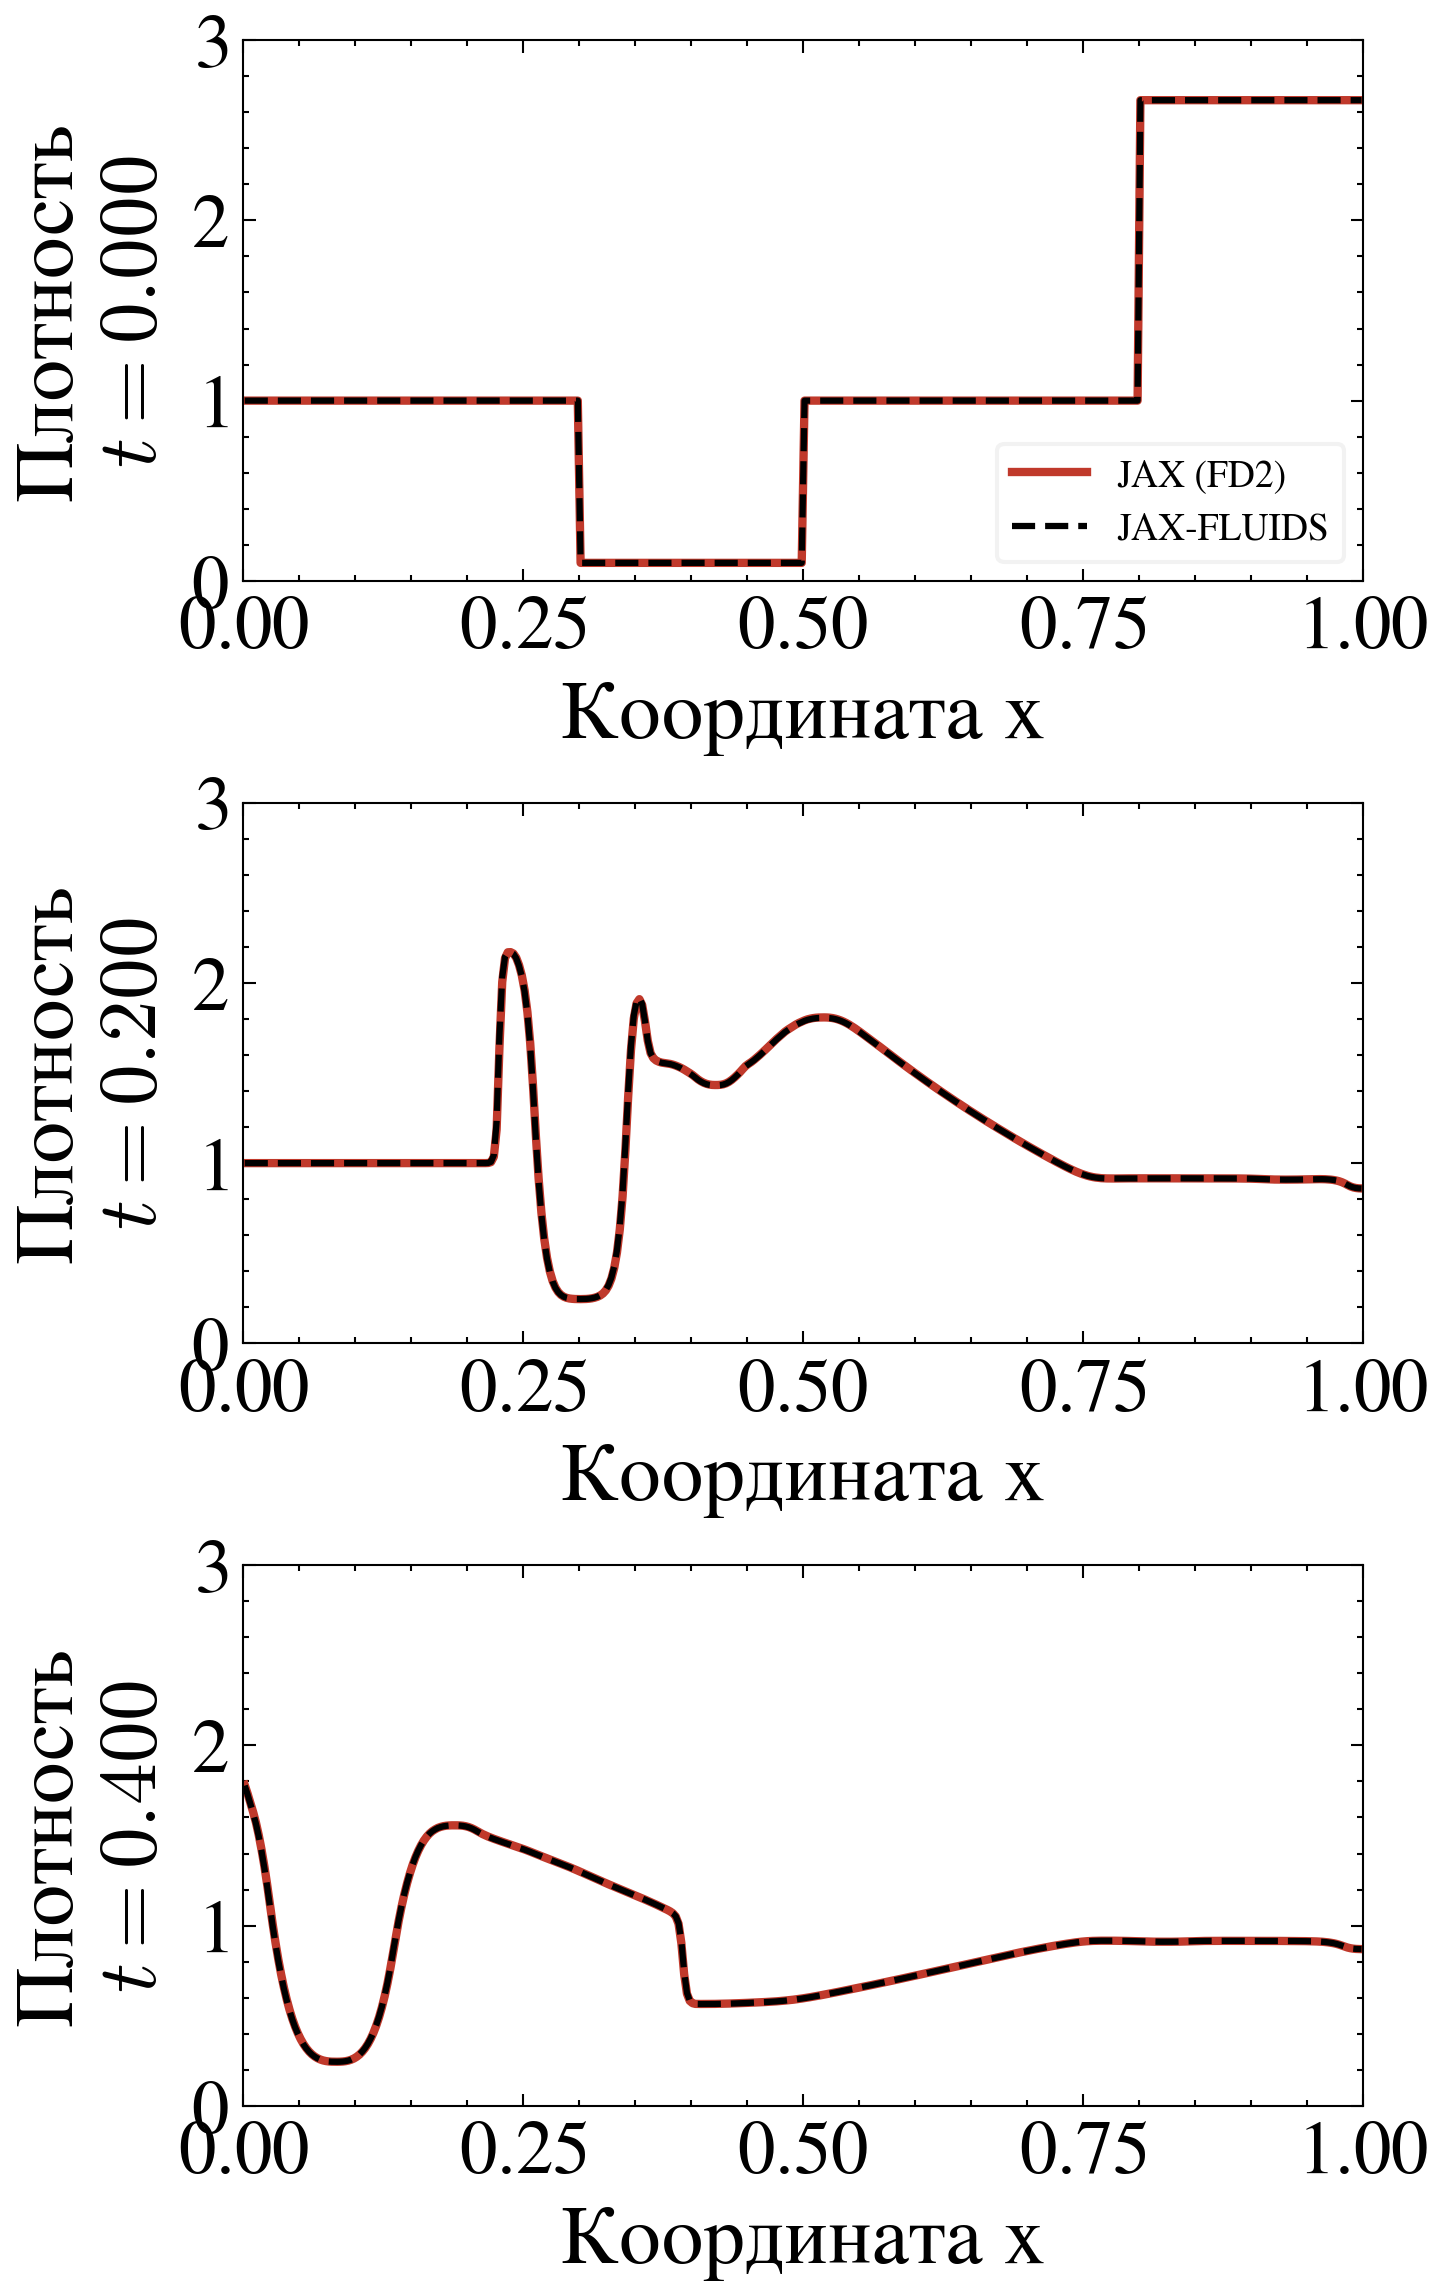
\includegraphics[width=1.06\textwidth]{rho_for_presentation_sd2_1d.png}
				
				\vspace{-0.25 cm}
				
				\caption*{\smaller{(a)}}
			\end{minipage}\hfill
			\begin{minipage}[t]{0.30\textwidth}
				\centering
				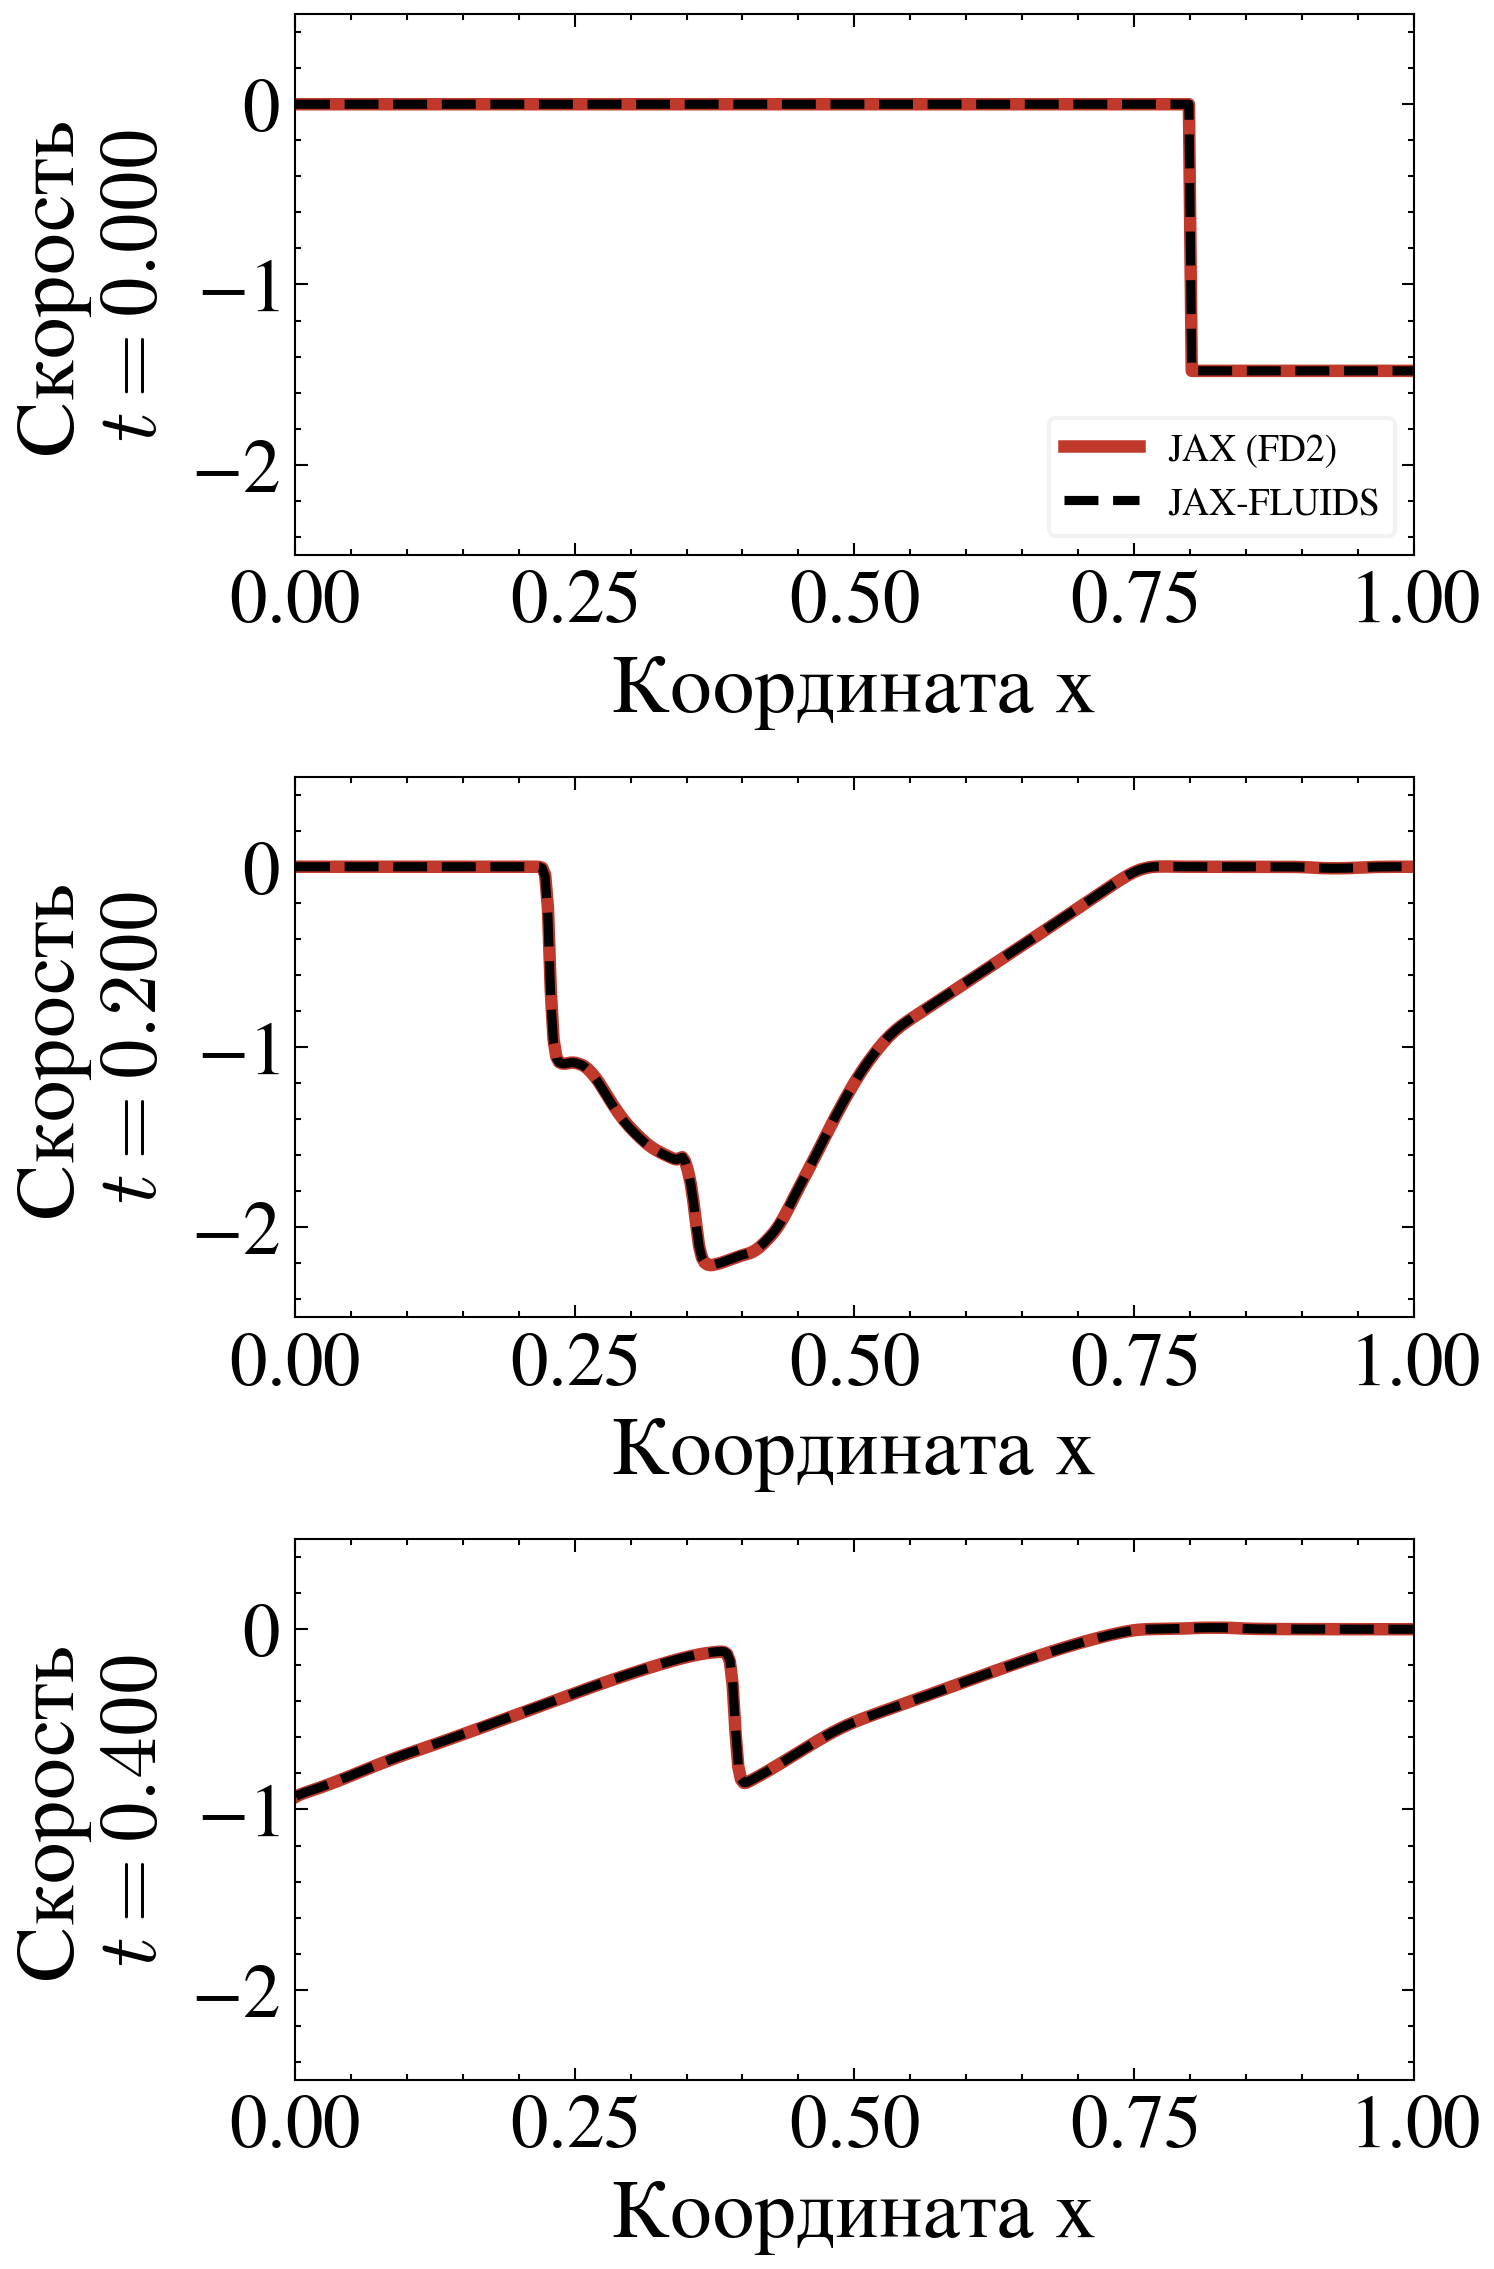
\includegraphics[width=\textwidth]{v_for_presentation_sd2_1d.png}
				
				\vspace{-0.25 cm}
				
				\caption*{\smaller{(b)}}
			\end{minipage}\hfill
			\begin{minipage}[t]{0.29\textwidth}
				\centering
				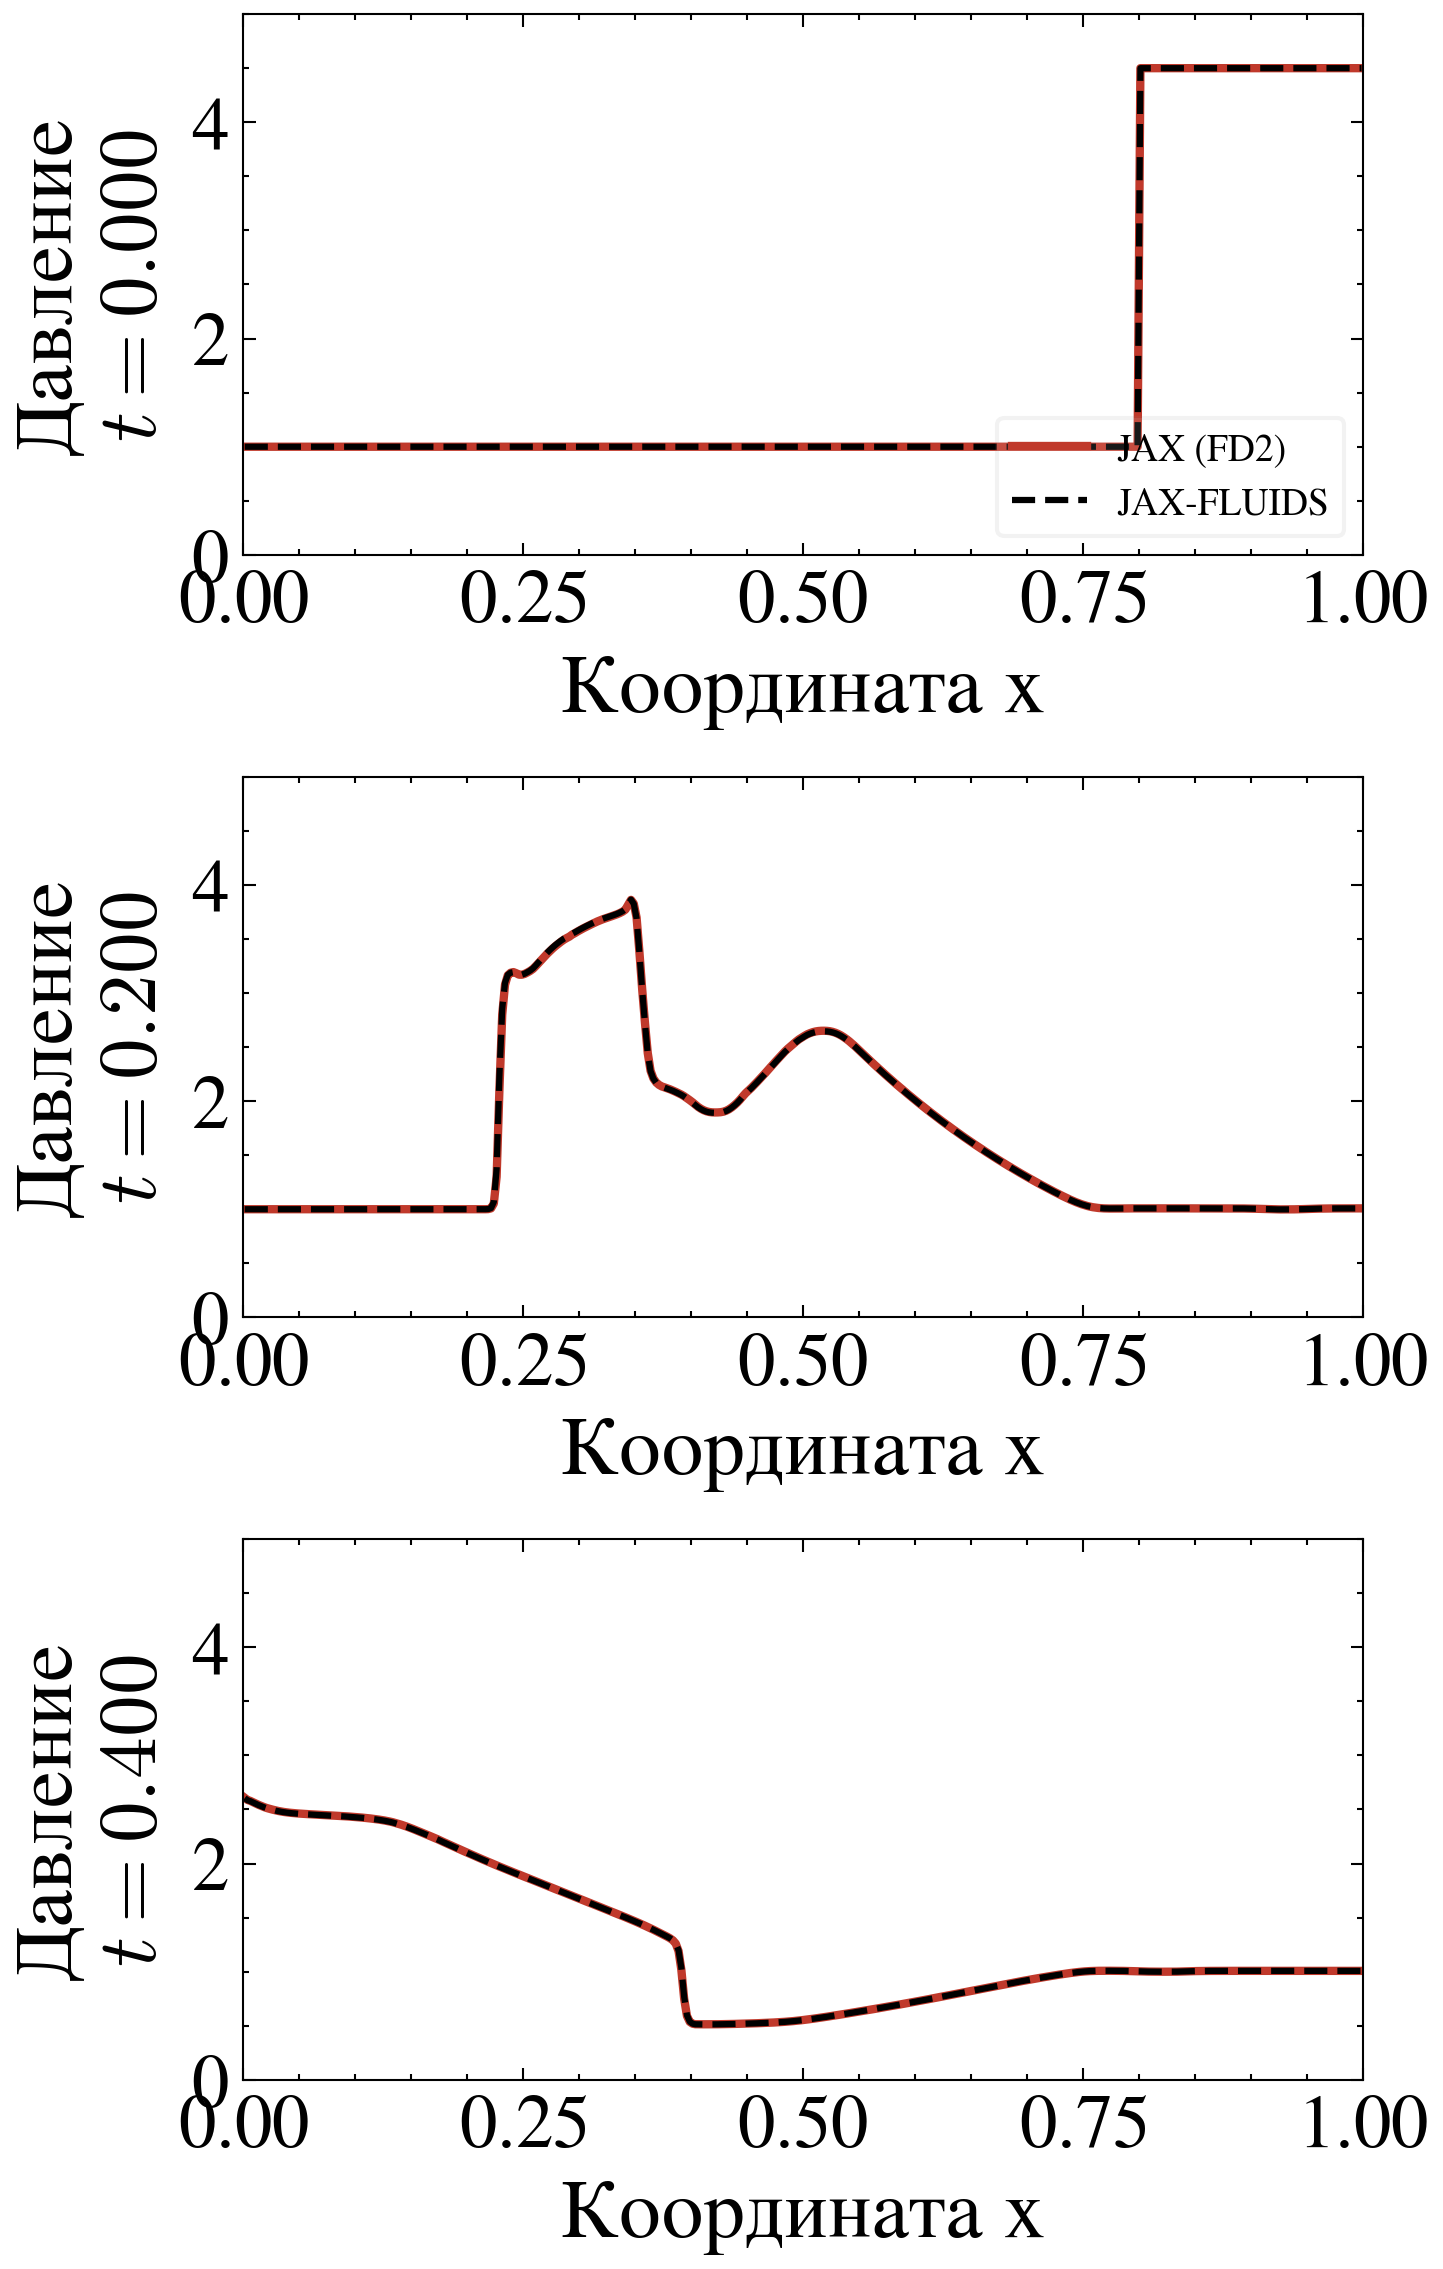
\includegraphics[width=\textwidth]{p_for_presentation_sd2_1d.png}
				
				\vspace{-0.25 cm}
				
				\caption*{\smaller{(c)}}
			\end{minipage}
			\vspace{-0.5 cm}
			\caption{ \smaller{Эволюция примитивных переменных в модифицированной 1D задаче Римана: (a) Плотность; (b) Скорость; (c) Давление с наложением на эталон \texttt{JAX-FLUIDS}}}
		\end{figure}

	\end{frame}

	%==================================================================
	% Слайд: Производительность (числа из диплома, 2D)
	\begin{frame}{Сравнительный анализ аппаратного ускорения: одномерная постановка}

		\begin{columns}[c]
			\begin{column}{0.5\textwidth}
				\begin{figure}[h]
					\centering
					\vspace{-0.3 cm}
					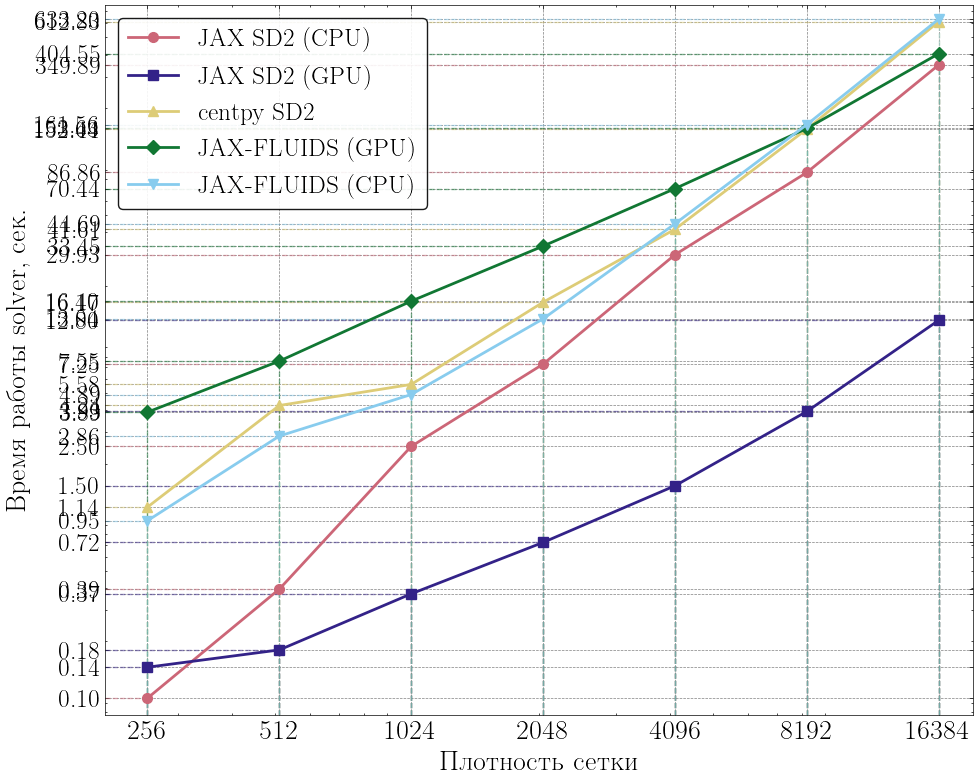
\includegraphics[width=\textwidth]{compare_plot_sd2_1d.png}
					\caption{\smaller{Время счёта (с) от размера сетки $J$ (1D, SD2), лог-лог.}}
				\end{figure}
			\end{column}
			\begin{column}{0.5\textwidth}
				\begin{table}[h]
					\centering
					\caption{\smaller{Время счёта (с), 1D, схема SD2}}
					\vspace{-0.3 cm}
					\resizebox{\textwidth}{!}{%
						\begin{tabular}{lccccc}
							\hline
							$J$ & \texttt{centpy} & Разраб. CPU & Разраб. GPU & JAX-FL. CPU & JAX-FL. GPU \\
							\hline
							$\mathbf{256}$   & 1.138   & 0.096   & \textbf{0.143}  & 0.954   & 3.894 \\
							$\mathbf{512}$   & 4.244   & 0.394   & \textbf{0.179}  & 2.857   & 7.545 \\
							$\mathbf{1024}$  & 5.577   & 2.499   & \textbf{0.370}  & 4.893   & 16.403 \\
							$\mathbf{2048}$  & 16.175  & 7.255   & \textbf{0.720}  & 13.040  & 33.451 \\
							$\mathbf{4096}$  & 41.613  & 29.928  & \textbf{1.500}  & 44.688  & 70.443 \\
							$\mathbf{8192}$  & 152.440 & 86.862  & \textbf{3.931}  & 161.556 & 153.630 \\
							$\mathbf{16384}$ & 612.826 & 349.892 & \textbf{12.805} & 633.204 & 404.548 \\
							\hline
						\end{tabular}
					}
				\end{table}
				\vspace{-0.2cm}
				\begin{alertblock}{}
					\small GPU (1D, $J=16384$): до $\mathbf{47.9\times}$ быстрее \texttt{centpy} и $\mathbf{27.3\times}$ быстрее собственной CPU-версии. На малых 1D-сетках выигрыш GPU невелик из-за накладных расходов (закон $T\propto J^2$); полное преимущество раскрывается в 2D.
				\end{alertblock}
			\end{column}
		\end{columns}
	\end{frame}

	%==================================================================
	% Слайд: 2D результаты (НОВЫЙ "вау"-слайд)
	\begin{frame}{Двумерная постановка задачи}

		\begin{block}{Система уравнений Эйлера (2D)}
			\[
			\partial_t \begin{pmatrix} \rho \\ \rho u \\ \rho v \\ \rho E \end{pmatrix} +
			\partial_x \begin{pmatrix} \rho u \\ \rho u^2 + p \\ \rho u v \\ (\rho E + p)u \end{pmatrix} +
			\partial_y \begin{pmatrix} \rho v \\ \rho u v \\ \rho v^2 + p \\ (\rho E + p)v \end{pmatrix} = 0
			\]
			с тем же уравнением состояния идеального газа $p = (\gamma - 1)\big(\rho E - \tfrac{1}{2}\rho (u^2 + v^2)\big)$, $\gamma = 1.4$.
		\end{block}

		в расчётной области $(x, y) \in [0, 1]^2$, с начальными условиями:
		\vspace{-0.15 cm}
		\[
		(\rho, u, v, p)|_{t=0} =
		\begin{cases}
			(2.667, -1.479, 0, 4.5) & \text{ударная волна: } x \in [0.8, 1], \\
			(\alpha \cdot 1, 0, 0, 1) & \text{зоны энерговложения,} \\
			(1, 0, 0, 1) & \text{фон (иначе).}
		\end{cases}
		\]

		\vspace{-0.2 cm}
		Две зоны пониженной плотности ($\alpha = 0.1$) --- круговая (центр $(0.45, 0.65)$, радиус $0.08$) и прямоугольная --- моделируют локальное энерговложение; УВ ($M_s = 2$) движется справа налево.

	\end{frame}
	
	%==================================================================
	% Слайд: Верификация (порядок точности)
	\begin{frame}{Анализ сходимости: гладкое решение (поправить для 2D)}
		\begin{block}{}
			Для верификации теоретического второго порядка точности схемы SD2 проведено моделирование эволюции уравнения линейного переноса.
			Порядок $p$ вычислялся методом экстраполяции Ричардсона с шагом измельчения $r=2$.
		\end{block}
		
		\begin{table}[h]
			\centering
			\footnotesize
			\renewcommand{\arraystretch}{1.3}
			\begin{tabular}{lccc}
				\hline
				\textbf{Переменная} & \textbf{Ошибка (100$\to$200)} & \textbf{Ошибка (200$\to$400)} & \textbf{Порядок $p$} \\
				\hline
				$u(x, t)$ & $8.92 \times 10^{-4}$ & $2.09 \times 10^{-4}$ & \textbf{2.09} \\
				\hline
			\end{tabular}
		\end{table}
		
		\begin{columns}[c]
			\begin{column}{0.55\textwidth}
				\[
				E = \|\mathbf{u}^{2h} - \mathbf{u}^{h}\|_{L_1} = \frac{1}{L} \sum_i |u_i^{2h} - u_i^h| \cdot \Delta x
				\]
				\[
				p = \log_2 \left( \frac{|| \mathbf{u}^{4h} - \mathbf{u}^{2h} ||_{L_1}}{|| \mathbf{u}^{2h} - \mathbf{u}^{h} ||_{L_1}} \right)
				\]
			\end{column}
			\begin{column}{0.45\textwidth}
				\footnotesize
				Неосцилляторность дополнительно подтверждена:
				\begin{itemize}
					\item контролем полной вариации $\mathrm{TV}(t)$ (1D);
					\item выполнением принципа максимума (2D).
				\end{itemize}
			\end{column}
		\end{columns}
		
	\end{frame}
	
		%==================================================================
	% Слайд: 1D результаты + кросс-верификация
	\begin{frame}{Численное решение: двумерная постановка}
		
		\begin{figure}[!h]
			\begin{minipage}[t]{0.27\textwidth}
				\centering
				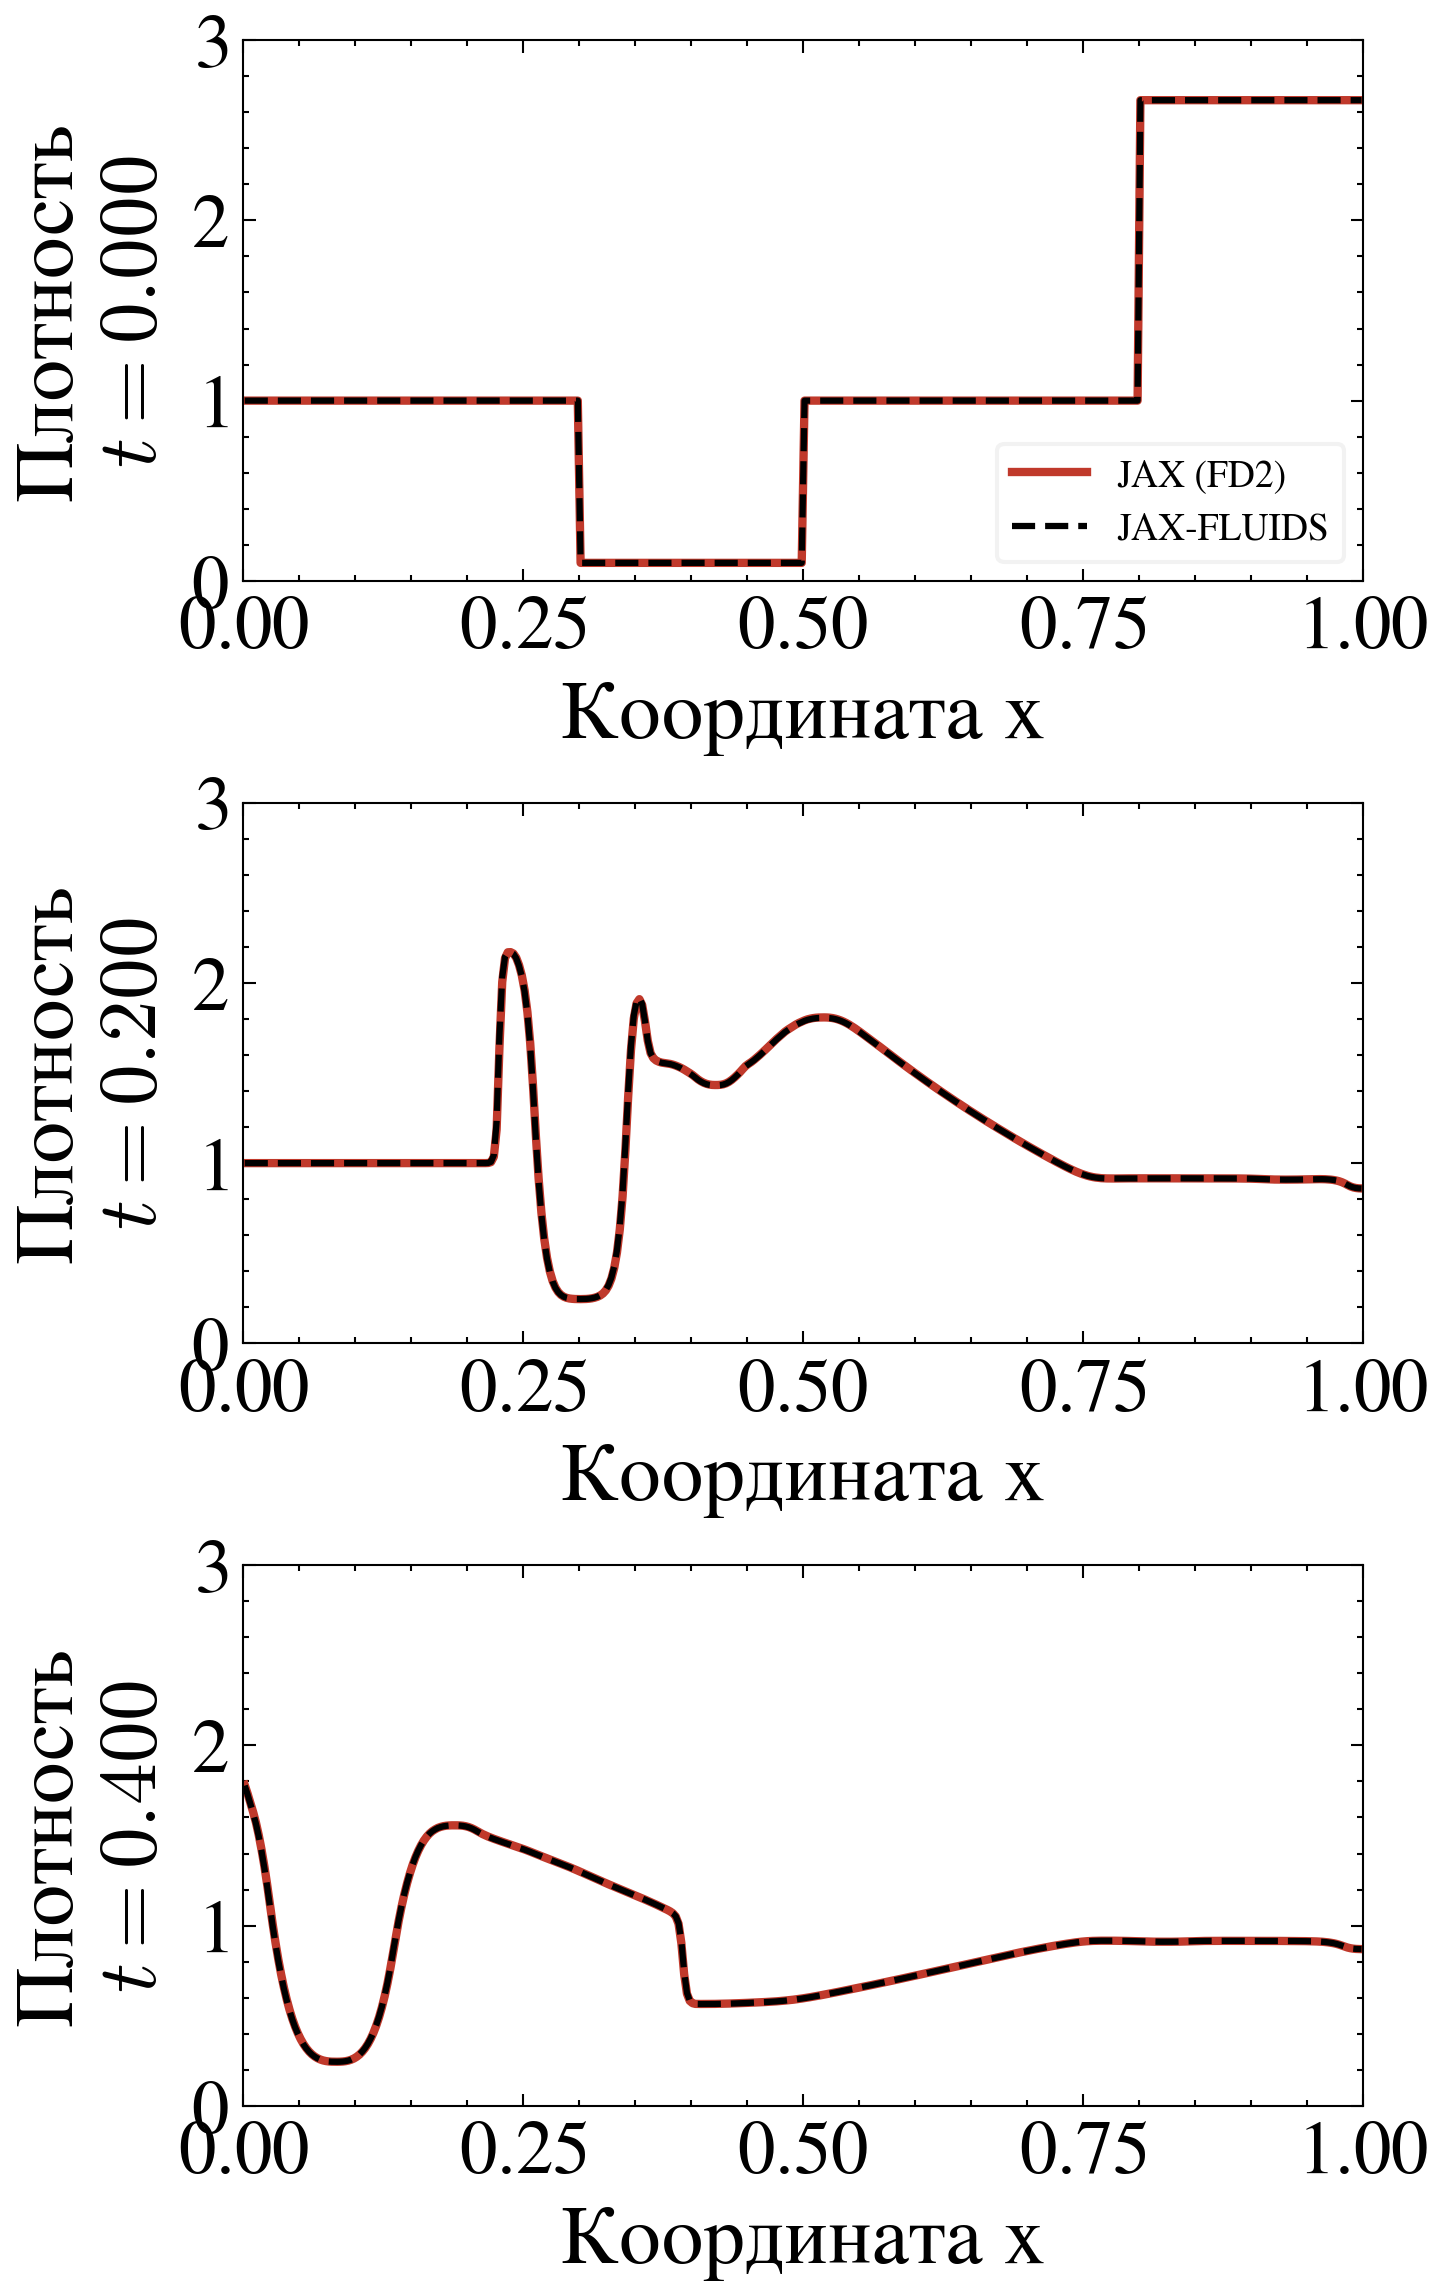
\includegraphics[width=1.06\textwidth]{rho_for_presentation_sd2_1d.png}
				
				\vspace{-0.25 cm}
				
				\caption*{\smaller{(a)}}
			\end{minipage}\hfill
			\begin{minipage}[t]{0.30\textwidth}
				\centering
				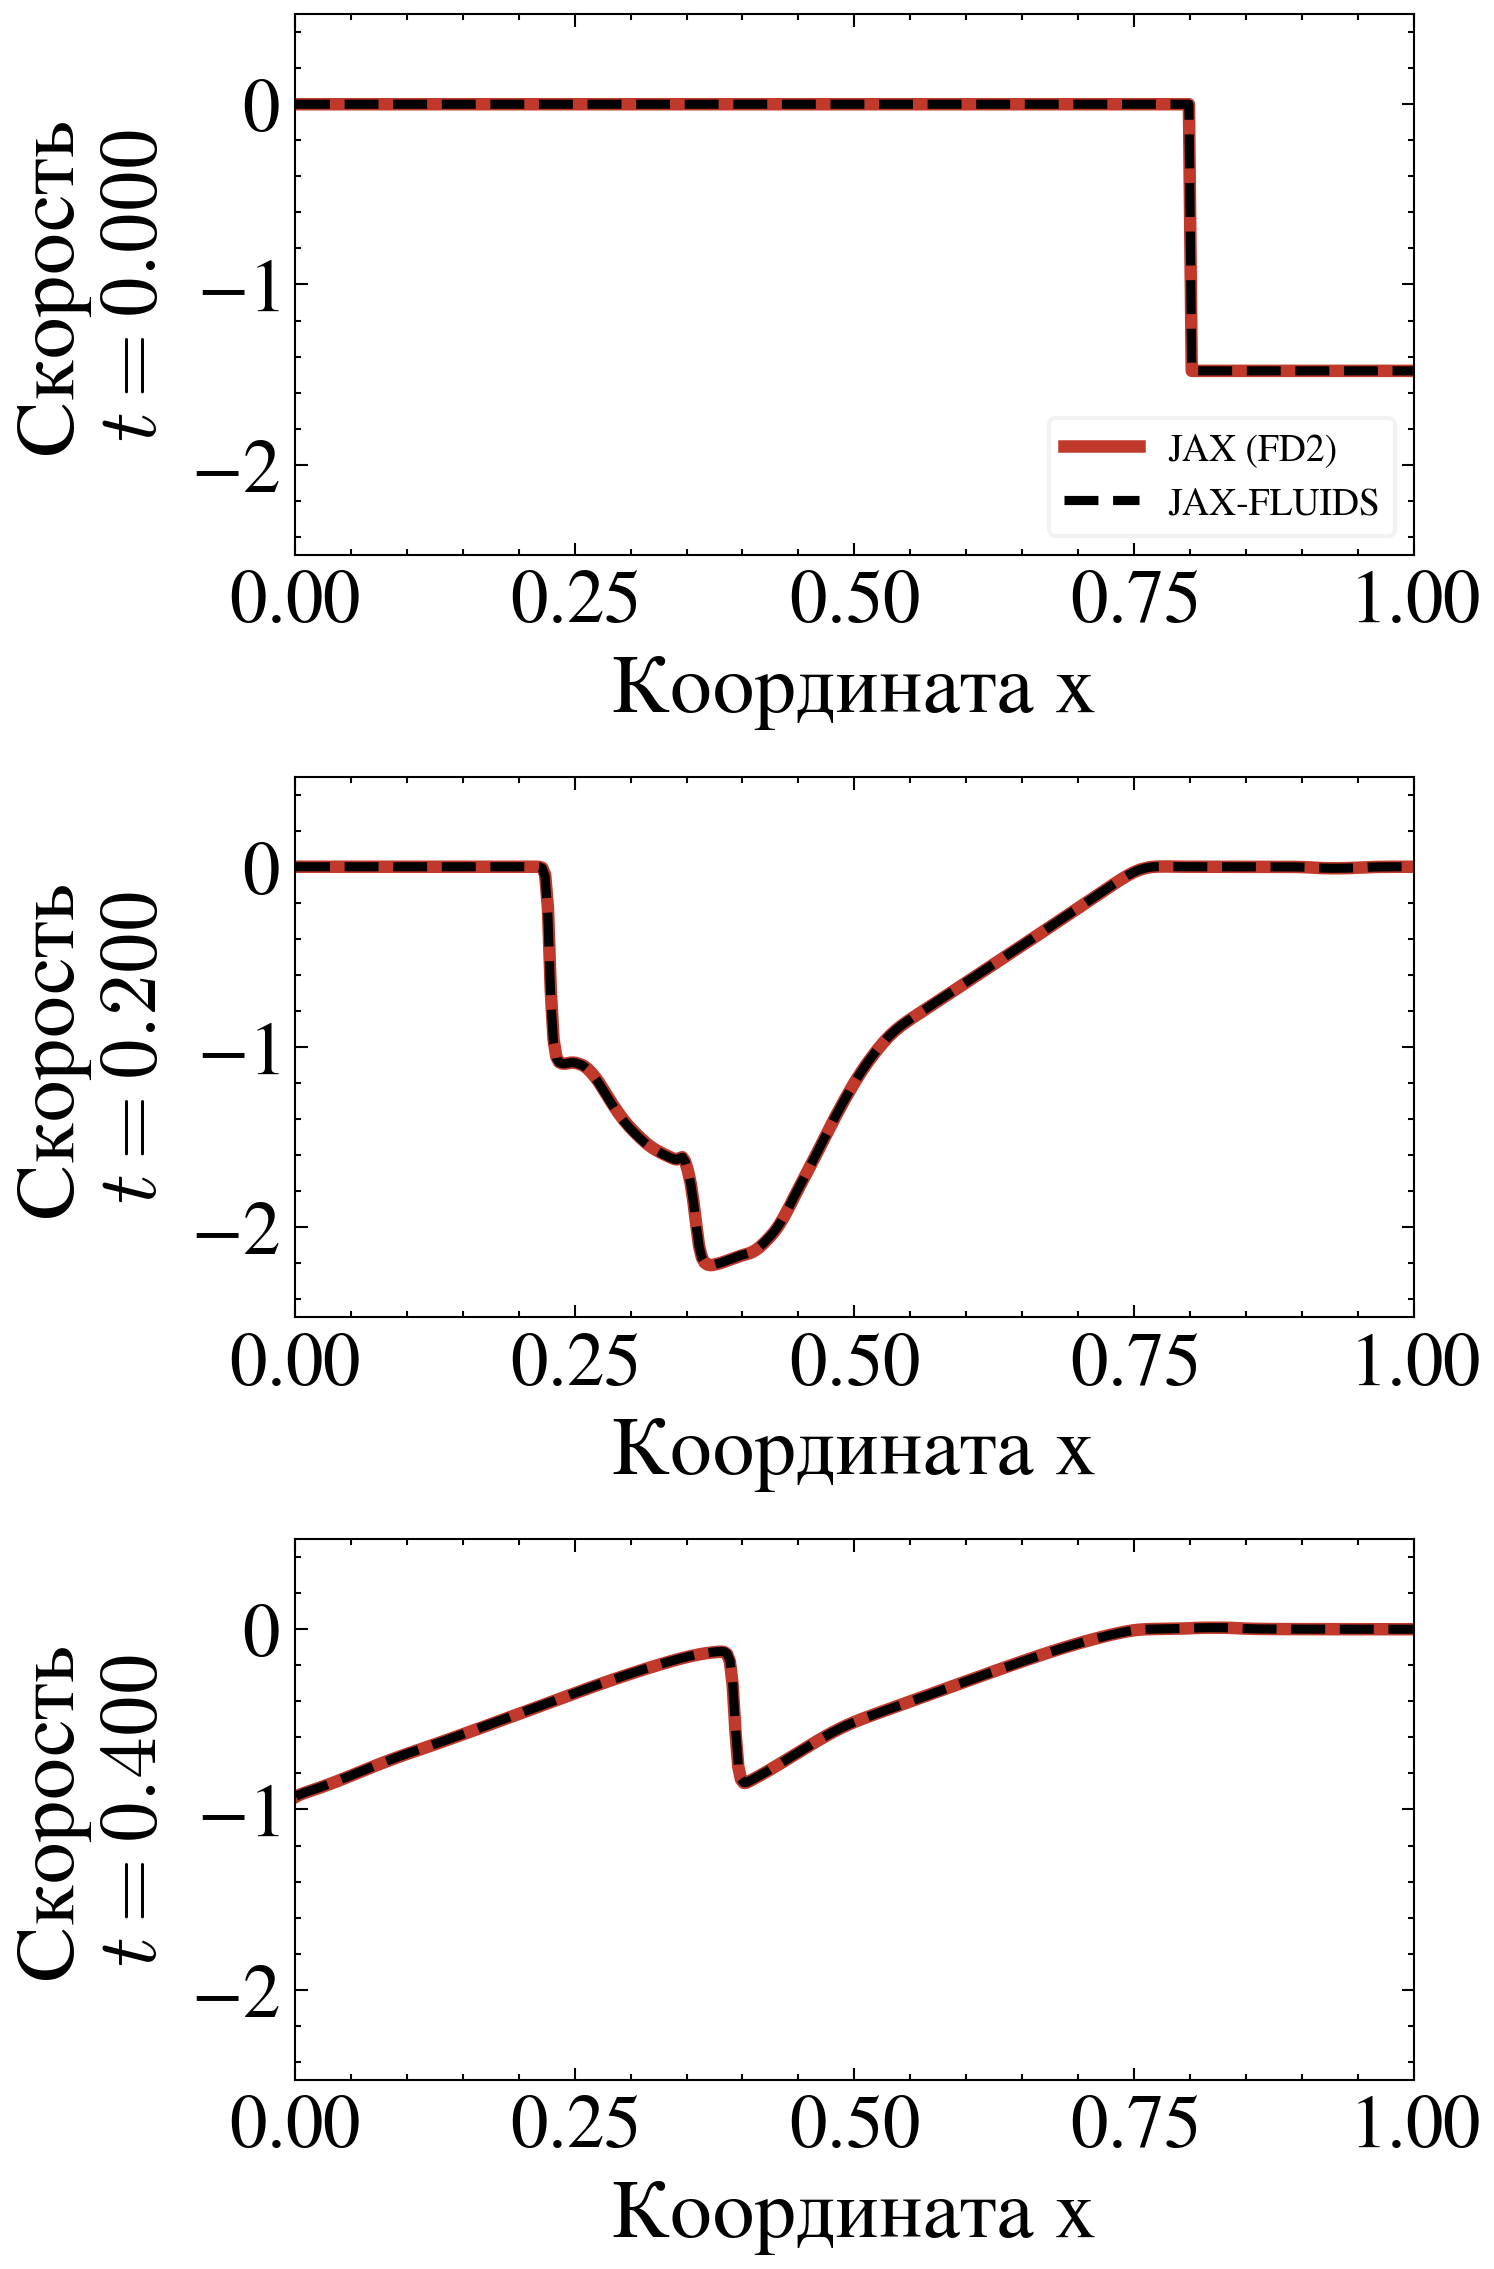
\includegraphics[width=\textwidth]{v_for_presentation_sd2_1d.png}
				
				\vspace{-0.25 cm}
				
				\caption*{\smaller{(b)}}
			\end{minipage}\hfill
			\begin{minipage}[t]{0.29\textwidth}
				\centering
				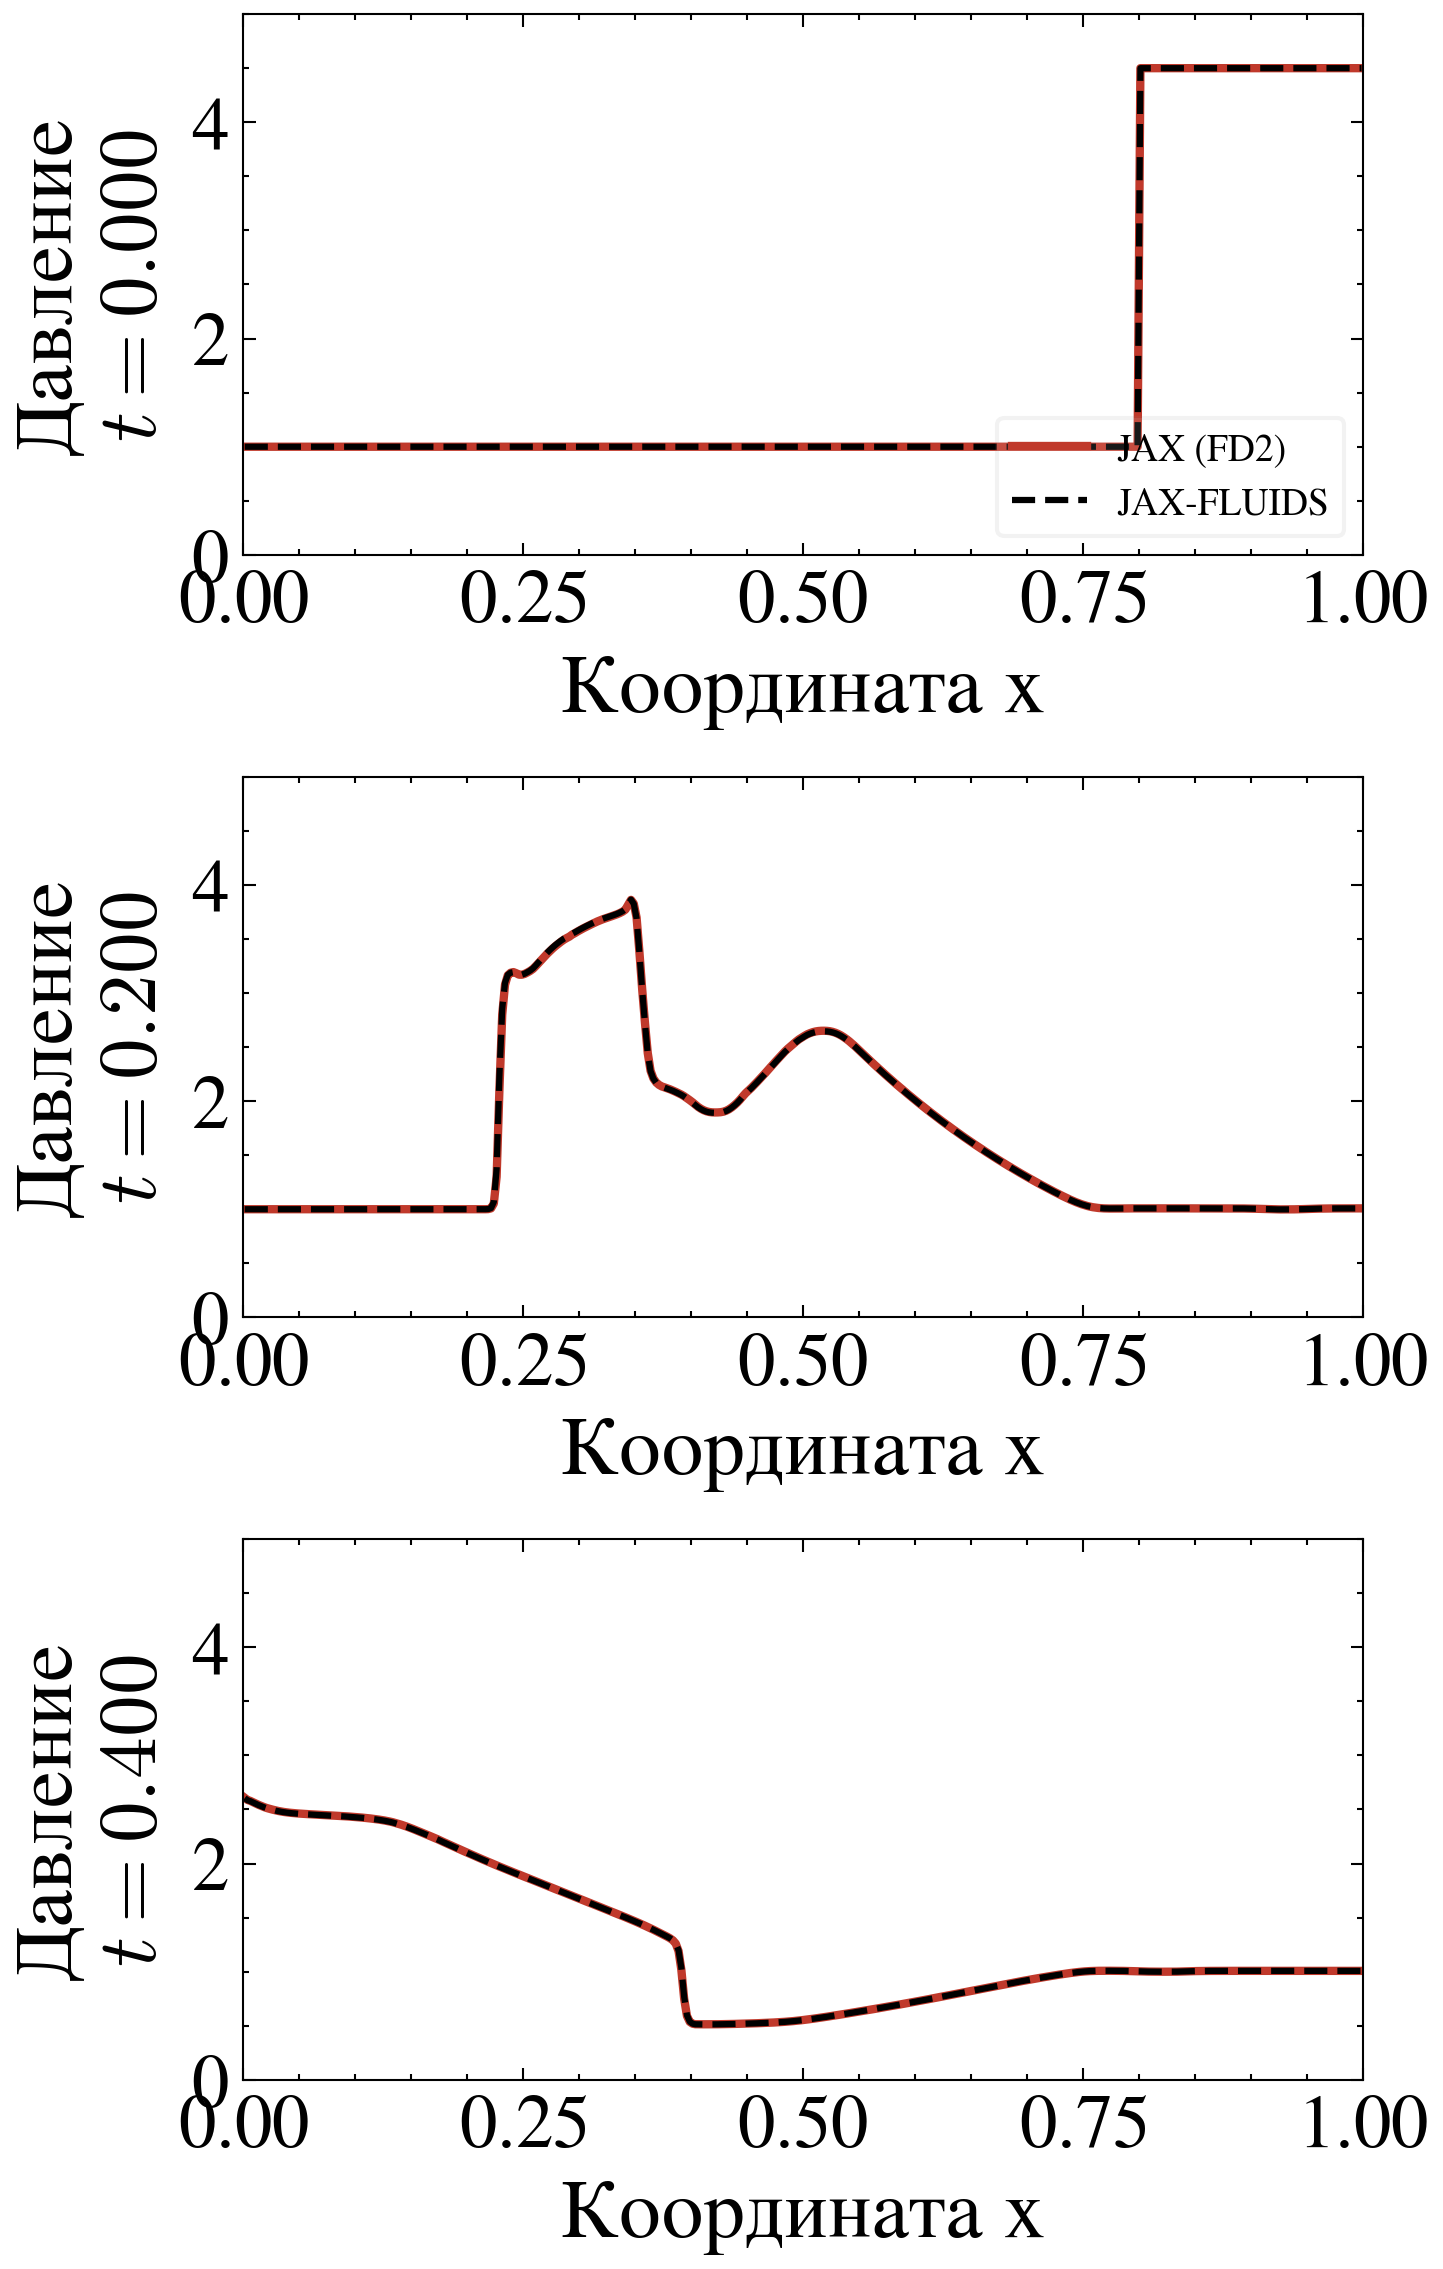
\includegraphics[width=\textwidth]{p_for_presentation_sd2_1d.png}
				
				\vspace{-0.25 cm}
				
				\caption*{\smaller{(c)}}
			\end{minipage}
			\vspace{-0.5 cm}
			\caption{ \smaller{Эволюция примитивных переменных в модифицированной 1D задаче Римана: (a) Плотность; (b) Скорость; (c) Давление с наложением на эталон \texttt{JAX-FLUIDS}}}
		\end{figure}
		
	\end{frame}

	%==================================================================
	% Слайд: Производительность (числа из диплома, 2D)
	\begin{frame}{Сравнительный анализ аппаратного ускорения: двумерная постановка}

		\begin{columns}[c]
			\begin{column}{0.5\textwidth}
				\begin{figure}[h]
					\centering
					\vspace{-0.3 cm}
					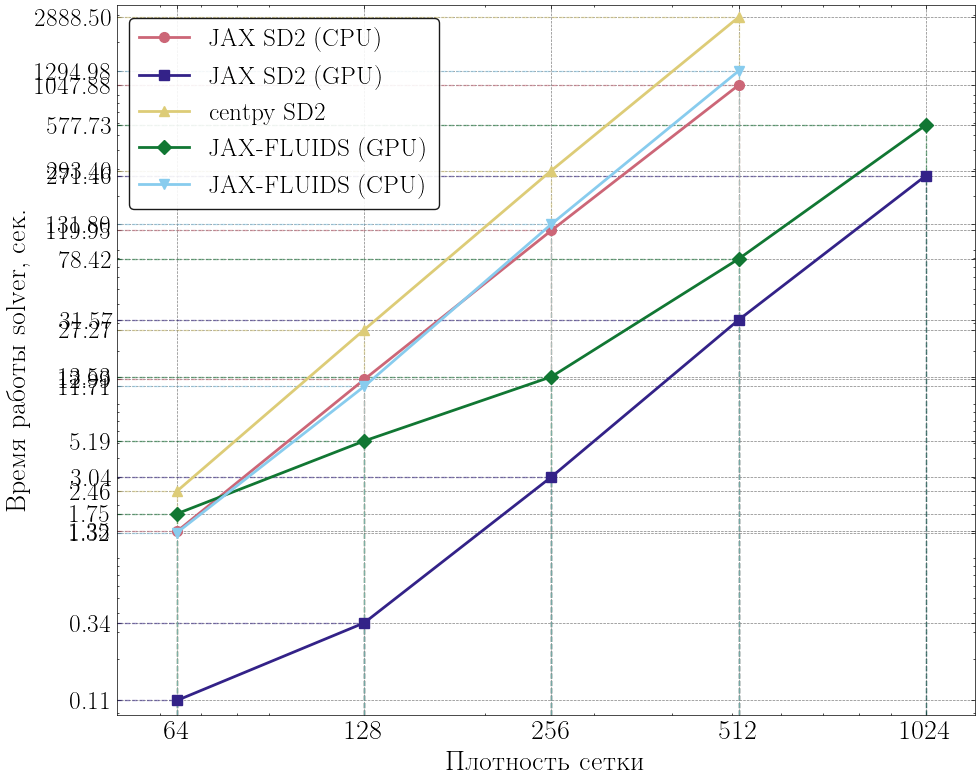
\includegraphics[width=\textwidth]{compare_plot_sd2_2d.png}
					\caption{\smaller{Время счёта (с) от размера сетки $J\times J$ (2D, SD2), лог-лог.}}
				\end{figure}
			\end{column}
			\begin{column}{0.5\textwidth}
				\begin{table}[h]
					\centering
					\caption{\smaller{Время счёта (с), 2D, схема SD2}}
					\vspace{-0.3 cm}
					\resizebox{\textwidth}{!}{%
						\begin{tabular}{lccccc}
							\hline
							$J\times J$ & \texttt{centpy} & Разраб. CPU & Разраб. GPU & JAX-FL. CPU & JAX-FL. GPU \\
							\hline
							$\mathbf{64}$   & 2.456    & 1.348    & \textbf{0.108}  & 1.322    & 1.753 \\
							$\mathbf{128}$  & 27.274   & 12.988   & \textbf{0.344}  & 11.709   & 5.191 \\
							$\mathbf{256}$  & 293.400  & 119.955  & \textbf{3.036}  & 131.803  & 13.530 \\
							$\mathbf{512}$  & 2888.498 & 1047.884 & \textbf{31.572} & 1294.979 & 78.417 \\
							$\mathbf{1024}$ & ---      & ---      & \textbf{271.457}& ---      & 577.726 \\
							\hline
						\end{tabular}
					}
				\end{table}
				\vspace{-0.2cm}
				\begin{alertblock}{}
					\small GPU (2D, $512\times512$): до $\mathbf{91.5\times}$ быстрее \texttt{centpy} и $\mathbf{33.2\times}$ быстрее собственной CPU-версии. Законы $T\propto J^2$ (1D), $T\propto J^3$ (2D).
				\end{alertblock}
			\end{column}
		\end{columns}

	\end{frame}

	%==================================================================
	% Слайд: Заключение (синхронно с дипломом, верные числа, смягчено)
	\begin{frame}{Заключение и основные результаты}

		\begin{block}{Выводы}
			\begin{enumerate}
				\item Поставлена и решена модифицированная задача Римана о прохождении УВ через зону энерговложения для уравнений Эйлера (1D и 2D).
				\item Реализован высокопроизводительный комплекс на базе \texttt{JAX} (схемы SD2 и FD2): JIT-компиляция, векторизация, единый код для CPU и GPU без модификации.
				\item Подтверждён второй порядок точности (экстраполяция Ричардсона); неосцилляторность --- через контроль $\mathrm{TV}$ и принцип максимума.
				\item Проведена кросс-верификация с точным решением, \texttt{centpy} и \texttt{JAX-FLUIDS}: достигнуто хорошее согласие профилей решений.
				\item В двумерных задачах решатель на GPU быстрее собственной CPU-реализации до $33\times$ (SD2) и $60\times$ (FD2), быстрее \texttt{centpy} в $90$--$100\times$, быстрее \texttt{JAX-FLUIDS} в $2.5$--$6\times$; достигнута сетка $1024\times1024$.
			\end{enumerate}
		\end{block}

	\end{frame}

	%==================================================================
	% ВСПОМОГАТЕЛЬНЫЕ СЛАЙДЫ
	\appendix

	\begin{frame}{Аппаратное ускорение вычислений: фреймворк JAX}
		Для преодоления вычислительных ограничений языка Python в качестве основы решателя выбран высокопроизводительный фреймворк JAX.

		\vspace{0.3cm}
		\textbf{Ключевые архитектурные преимущества:}
		\begin{itemize}
			\item \textbf{JIT-компиляция (Just-In-Time):} компилятор XLA (Accelerated Linear Algebra) транслирует высокоуровневый код Python в оптимизированные машинные инструкции.
			\item \textbf{Глубокая векторизация:} отказ от явных циклов по пространственной сетке; массивы обрабатываются параллельно на уровне тензорных операций.
			\item \textbf{Кроссплатформенность:} единый код (математическая логика решателя) нативно и без модификаций выполняется на многоядерных CPU и графических ускорителях (GPU/TPU).
		\end{itemize}
	\end{frame}

	\begin{frame}{Семейство численных схем Курганова--Тадмора}

		\begin{block}{Основные особенности метода:}
			\begin{itemize}
				\item \textbf{Вычисление потоков:} потоки на гранях ячеек определяются без вычисления матриц Якоби и характеристических переменных.
			\end{itemize}
		\end{block}

		\begin{block}{Подходы к дискретизации:}
			\begin{itemize}
				\item \textbf{Fully-Discrete (FD):} пространственный и временной шаги жёстко связаны единым вычислительным шаблоном.
				\item \textbf{Semi-Discrete (SD):} пространственная дискретизация сводит УЧП к системе ОДУ (метод прямых). Интегрирование по времени выполняется независимыми TVD-схемами Рунге--Кутты. Различают схемы 2-го (SD2) и 3-го (SD3) порядка точности.
			\end{itemize}
		\end{block}

	\end{frame}

	\begin{frame}{Пространственная реконструкция схемы SD2}

		\begin{block}{TVD-свойство (Total Variation Diminishing)}
			Схема не порождает новые локальные экстремумы, если
			\vspace{-0.2 cm}
			\[
			TV(u^{n+1}) \leq TV(u^{n}),
			\]
			где общая вариация решения $TV(u) = \sum_{i = 1}^{N - 1} |u_{i + 1}(t) - u_i(t)|$
		\end{block}

		Для обеспечения TVD-свойства используются нелинейные ограничители наклонов (limiter):
		\vspace{-0.3 cm}
		\[
		\text{minmod}(a,b) = \frac{1}{2} \big( \operatorname{sgn}(a) + \operatorname{sgn}(b) \big) \cdot \min\big( |a|, |b| \big).
		\]
	\end{frame}

	% Бэкап: 1D-производительность
	\begin{frame}{Производительность: одномерная задача (бэкап)}
		\begin{table}[h]
			\centering
			\footnotesize
			\caption{\smaller{Время счёта (с), 1D, схема SD2}}
			\vspace{-0.2 cm}
			\resizebox{\textwidth}{!}{%
				\begin{tabular}{lccccc}
					\hline
					$J$ & \texttt{centpy} & Разраб. CPU & Разраб. GPU & JAX-FL. CPU & JAX-FL. GPU \\
					\hline
					$\mathbf{256}$   & 1.138   & 0.096   & \textbf{0.143}  & 0.954   & 3.894 \\
					$\mathbf{512}$   & 4.244   & 0.394   & \textbf{0.179}  & 2.857   & 7.545 \\
					$\mathbf{1024}$  & 5.577   & 2.499   & \textbf{0.370}  & 4.893   & 16.403 \\
					$\mathbf{2048}$  & 16.175  & 7.255   & \textbf{0.720}  & 13.040  & 33.451 \\
					$\mathbf{4096}$  & 41.613  & 29.928  & \textbf{1.500}  & 44.688  & 70.443 \\
					$\mathbf{8192}$  & 152.440 & 86.862  & \textbf{3.931}  & 161.556 & 153.630 \\
					$\mathbf{16384}$ & 612.826 & 349.892 & \textbf{12.805} & 633.204 & 404.548 \\
					\hline
				\end{tabular}
			}
		\end{table}
		\centering\small
		Ускорение GPU (1D, $J=16384$): $47.9\times$ относительно \texttt{centpy}, $27.3\times$ относительно собственной CPU-версии.
		На малых 1D-сетках выигрыш GPU невелик из-за накладных расходов; преимущество раскрывается в 2D.
	\end{frame}

\end{document}
